\section{Typical Simulation}
Is Typical\_simulation.tex needed in this section?
If anything it would be the sanity check simulations


The system
  \begin{align}
    M_t &= \nabla_x \left( D(M) \nabla_x M \right) + f(C,M) M \\
    C_t &= - g(C,M) 
  \end{align}
  where
  \begin{align}
    D(M) &= \delta \frac{M^\alpha}{(1 - M)^\beta} \\
    f(C,M) &= \frac{ C }{{k } + {C}} \left(1 - \left( \frac{M M_0}{{C C_0 + \epsilon}} \right)^\gamma \right) \\
    g(C,M) &= \frac{\nu C}{k +C} M
  \end{align}
  is solved on a rectangular region with length $L$ and width $\lambda L$ with the following parameter values,
  \begin{equation}
    \begin{aligned}
      L &= 0.01 \\
      \lambda &= \frac{1}{128}\\
      \epsilon &= 10^{-8}\\
      \alpha &= 4 \\
      \beta &= 4 \\
      \gamma &= 0.5 \\
      \mu &= 6 \\      
    \end{aligned}
    \qquad
    \begin{aligned}
      C_0 &= 30 \\
      M_0 &= 30 \\
      \delta &= \frac{10^{-7}}{\mu L^2} \approx 10^-4\\
      k &= \frac{4}{C_0} \approx 0.1333\\
      \nu &= \frac{M_0}{0.63 C_0} \approx 1.59,\\
    \end{aligned}
  \end{equation}
  and with initial conditions 
  \begin{equation}
    \begin{aligned}
      C &= 1 \\
      M &= \begin{cases} -(\frac{h}{d^4})x^4 + h & \text{if } x < 0.04 \\ 0 & \text{otherwise }\end{cases} \\
    \end{aligned}
  \end{equation}  
  where $h = 0.05, d=0.04$ , representing the height and depth of the inoculation site.

  A series of test was done on simulation code version $0.1.1$. These were defaulted to run with $\Delta t = 10^{-3}$ and $\Delta x = \frac{1}{256}$.
  
  The following lists the test, and observations from each.
  
  \begin{enumerate}
    \item Solve the system with homogenous initial conditions and see if it stays homogenous.
      \begin{itemize}
        \item Worked!
        \item The biomass and substrate concentration at $t=8$ did not change as grid size did, which is good. 
        \item Biomass and substrate concentration did change for step size, but it was converging to a specific value (Table \ref{tab:homoIC}), which makes sense and suggests that default choice of $\Delta t$ is good.
        \begin{table}
          \begin{center}
            \begin{tabular}{| c | c | c |}
              \hline
              $\Delta t$ & Biomass Density & Substrait Conc. \\
              \hline
              $10^{-1}$ & 0.743806469443 & 0.731575100108\\
              $10^{-2}$ & 0.739180637812 & 0.736539504220\\
              $10^{-3}$ & 0.738699851204 & 0.737025027162 \\
              $10^{-4}$ & 0.738651598939 & 0.737073472750\\
              $10^{-5}$ & 0.738646771985 & 0.737078316244\\
              \hline
            \end{tabular}
            \caption{Values of biomass and substrate concentration at $t = 8$. A grid size of $\Delta x = 1/256$ was used.}
            \label{tab:homoIC}
          \end{center}
        \end{table}
      \end{itemize}

%    \item Solve the system with non-homogenous high initial condition ($M_0=0.95$), with zero forcing term, and see if density-dependent diffusion moves it without loss of biomass.
%      \begin{itemize}
%        \item DOESN"T WORK!!!!!!
%      \end{itemize}
  
      
    \item Solve the system with $f = s$, $s$ a constant, and see if total biomass follows $be^{st}$, where $b$ is the initial total biomass.
    \begin{itemize}
      \item Works with $D(M) = 0$.
      
      \item With $D(M) = \delta$ total biomass grows a little slower then $be^{st}$ which becomes slightly noticable at later times. The difference is less then 1\%, so this looks good. See Figure \ref{fig:totalBioCheck}(ab).
      
      \item With $D(M) = \delta M^{\alpha}$ the total biomass matchs $be^{st}$ until the biomass density at the innoculation point becomes greater then 1. Since physically this should never occur, this isn't a problem.  See Figure \ref{fig:totalBioCheck}(c).
      
      \item With $D(M) = \frac{\delta M^{\alpha}}{(1-M)^\beta}$ the total biomass grows accuratly until it approches $M \in (0.9, 1)$ at the innoculation point. This is a problem, because at this point the density dependent diffusion should start and keep the solution growing with $be^{st}$. This suggests that there is something wrong with how the diffusion is being implemented, will follow up on this.  See Figure \ref{fig:totalBioCheck}(d).
      
      \begin{figure}
        \begin{center}
          \begin{tabular}{c c}
            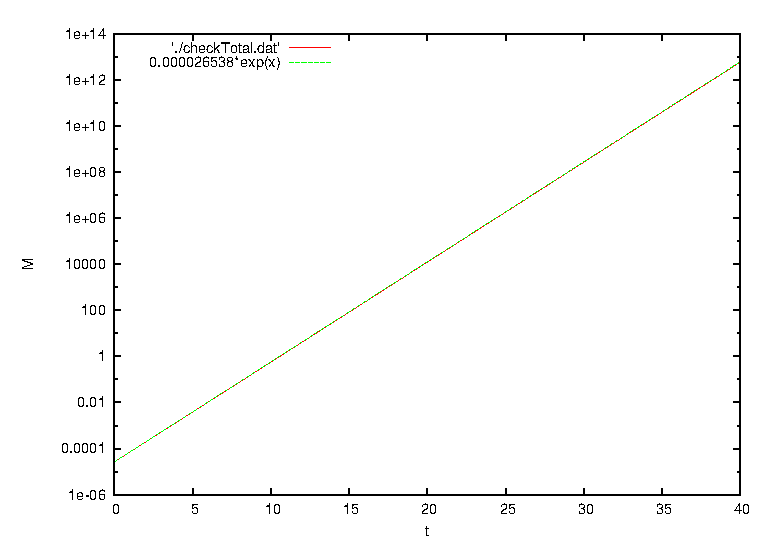
\includegraphics[scale=0.5]{checkTotal_Dconstant.eps} &
            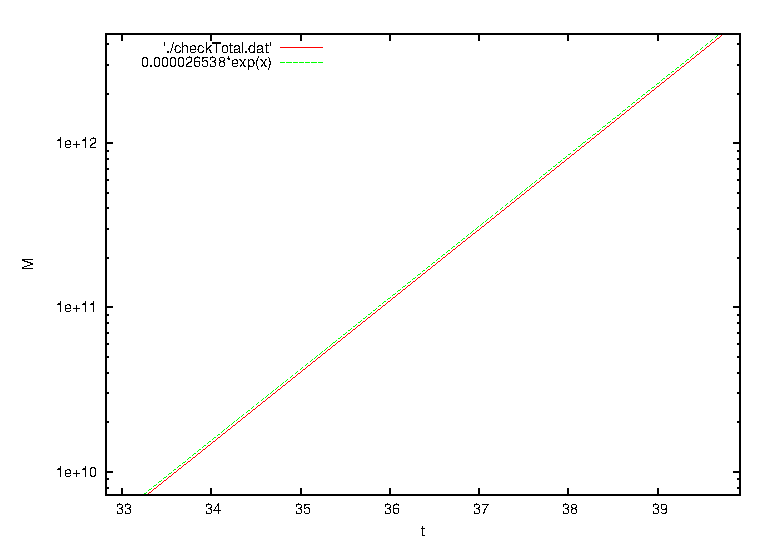
\includegraphics[scale=0.5]{checkTotal_Dconstant_zoomed.eps} \\
            (a) & (b) \\
            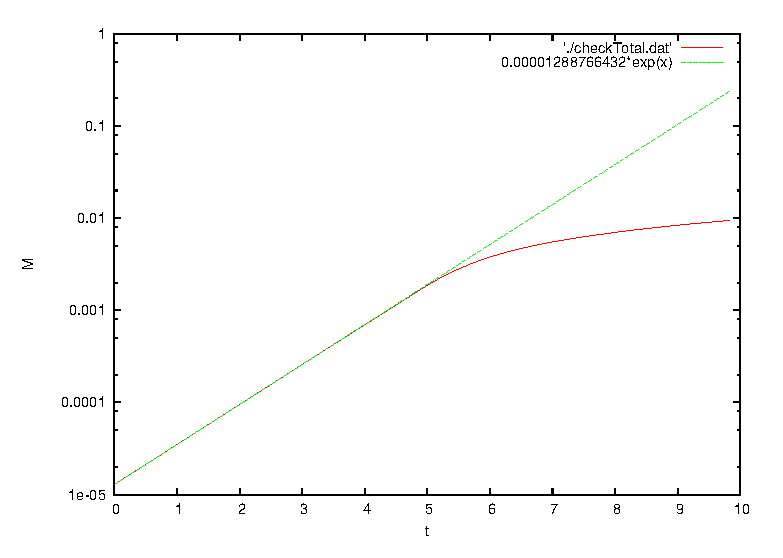
\includegraphics[scale=0.5]{checkTotal_Dporous.eps} & 
            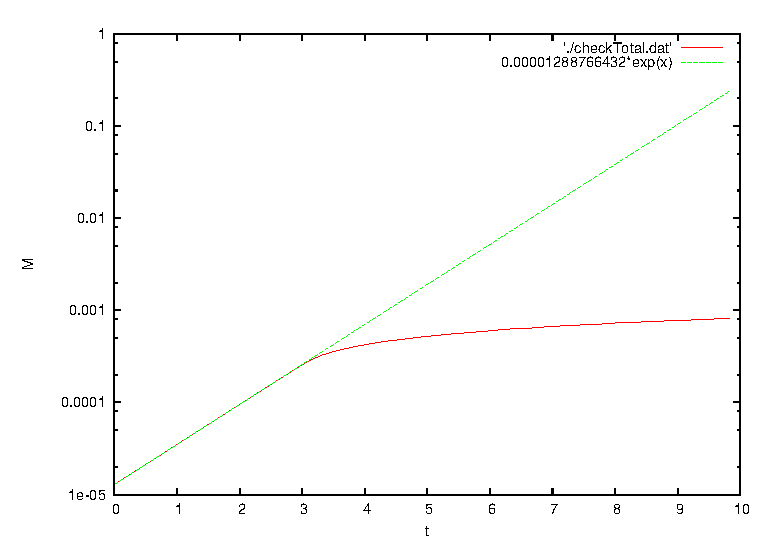
\includegraphics[scale=0.5]{checkTotal_Ddensity.eps} \\
            (c) & (d) \\
          \end{tabular}
          \captionsetup{singlelinecheck=off}
          \caption[enum]{Graph of, 
            \begin{enumerate}[(a)]
              \item $D(M) = \delta$, 
              \item $D(M) = \delta$; zoomed in to show the slight difference in growth,
              \item $D(M) = \delta M^\alpha$,
              \item $D(M) = \frac{\delta M^{\alpha}}{(1-M)^\beta} $.
            \end{enumerate} 
          }

          \label{fig:totalBioCheck}
        \end{center}
      \end{figure}
      
    \end{itemize}
      
  \end{enumerate}
